%pdflatex main.tex
%bibtex main
%pdflatex main.tex
%pdflatex main.tex

% Based on the course template (2026-2027/Report/texModel/model.tex).
% Changes to the template: utf8 input (author names with diacritics), tikz/booktabs/tabularx
% for the graphical abstract and tables, and the plainurl bibliography style (plain + DOI/URL).

\documentclass[runningheads,a4paper,11pt]{report}

\usepackage{algorithmic}
\usepackage{algorithm}
\usepackage{array}
\usepackage{amsmath}
\usepackage{amsfonts}
\usepackage{amssymb}
\usepackage{amsthm}
\usepackage{caption}
\usepackage{comment}
\usepackage{epsfig}
\usepackage{fancyhdr}
\usepackage[T1]{fontenc}
\usepackage{geometry}
\usepackage{graphicx}
\usepackage[colorlinks]{hyperref}
\usepackage[utf8]{inputenc}
\usepackage{multicol}
\usepackage{multirow}
\usepackage{rotating}
\usepackage{setspace}
\usepackage{subfigure}
\usepackage{url}
\usepackage{verbatim}
\usepackage{xcolor}
\usepackage{booktabs}
\usepackage{tabularx}
\usepackage{pgfgantt}
\usepackage{tikz}
\usetikzlibrary{arrows.meta,positioning,fit,backgrounds,calc}
\usepackage{titlesec}

% compact chapter headings that do not start a new page (keeps the milestone report short)
\titleclass{\chapter}{straight}
\titleformat{\chapter}{\normalfont\LARGE\bfseries}{\thechapter}{0.8em}{}
\titlespacing*{\chapter}{0pt}{18pt}{10pt}

\geometry{a4paper,top=3cm,left=2cm,right=2cm,bottom=3cm,headheight=24pt}

\pagestyle{fancy}
\fancyhf{}
\fancyhead[LE,RO]{Cardiac Digital Twin from Wearable Sensors}
\fancyhead[RE,LO]{Team \teamname}
\fancyfoot[RE,LO]{Advanced Machine Learning --- 2026-2027}
\fancyfoot[LE,RO]{\thepage}

\renewcommand{\headrulewidth}{2pt}
\renewcommand{\footrulewidth}{1pt}
\renewcommand{\headrule}{\hbox to\headwidth{%
  \color{lime}\leaders\hrule height \headrulewidth\hfill}}
\renewcommand{\footrule}{\hbox to\headwidth{%
  \color{lime}\leaders\hrule height \footrulewidth\hfill}}

% ---- team placeholders: fill these in -------------------------------------------
\newcommand{\teamname}{[team name]}
\newcommand{\memberA}{[Member A]}
\newcommand{\memberB}{[Member B]}
\newcommand{\memberC}{[Member C]}
% ---------------------------------------------------------------------------------

\hypersetup{
pdftitle={AI-Enabled Cardiac Digital Twin from Wearable Sensors},
pdfauthor={\teamname},
pdfkeywords={digital twin, ECG, wearable, arrhythmia, denoising, transformers, multi-agent systems},
bookmarksnumbered,
pdfstartview={FitH},
urlcolor=cyan,
colorlinks=true,
linkcolor=red,
citecolor=green,
}

\newcommand{\R}{\mathbb{R}}
\newcommand{\twin}{\mathcal{T}}

\setcounter{secnumdepth}{3}
\setcounter{tocdepth}{0}
\linespread{1}
\makeindex


\begin{document}

\begin{titlepage}
\sloppy

\begin{center}
BABE\c S BOLYAI UNIVERSITY, CLUJ NAPOCA, ROM\^ ANIA

FACULTY OF MATHEMATICS AND COMPUTER SCIENCE

\vspace{5cm}

\Huge \textbf{AI-Enabled Cardiac Digital Twin\\from Wearable Sensors}

\vspace{0.6cm}

\Large Personalised, multi-agent monitoring of single-lead ECG

\vspace{1cm}

\normalsize -- Advanced Machine Learning report --

\vspace{0.3cm}

\normalsize Milestone 1 (Seminar 3): problem description and survey of related work

\end{center}


\vspace{4cm}

\begin{flushright}
\Large{\textbf{Authors}}\\
\normalsize
\memberA, [specialisation], [group], [email]\\
\memberB, [specialisation], [group], [email]\\
\memberC, [specialisation], [group], [email]
\end{flushright}

\vspace{3cm}

\begin{center}
2026-2027
\end{center}

\end{titlepage}

\pagenumbering{gobble}

\section*{Team}

\begin{center}
\small
\setstretch{1.1}
\begin{tabularx}{\textwidth}{@{}>{\raggedright\arraybackslash}p{4.4cm}>{\raggedright\arraybackslash}X>{\raggedright\arraybackslash}p{5.0cm}@{}}
\toprule
\textbf{Member} & \textbf{Role} & \textbf{Milestone 1 tasks} \\
\midrule
\memberA, [email], [specialisation] & Signal Monitoring agent, data pipeline & Survey: wearable ECG, denoising \\
\memberB, [email], [specialisation] & Arrhythmia Detection and Physiological Prediction agents & Survey: classification, forecasting \\
\memberC, [email], [specialisation] & Twin Calibration and Clinical Recommendation agents & Problem definition; survey: twins, agents \\
\bottomrule
\end{tabularx}
\end{center}

\begin{center}
\begin{ganttchart}[
  hgrid,
  vgrid={*1{dotted}},
  x unit=2.3cm,
  y unit title=0.5cm,
  y unit chart=0.42cm,
  title height=1,
  bar height=0.6,
  bar top shift=0.2,
  bar/.append style={fill=blue!25},
  bar label font=\scriptsize,
  title label font=\scriptsize\bfseries,
]{1}{4}
\gantttitle{Seminar 3}{1} \gantttitle{Seminar 4}{1} \gantttitle{Seminar 6}{1} \gantttitle{Seminar 7}{1} \\
\ganttbar[bar/.append style={fill=green!45}]{Problem definition, literature review (all)}{1}{1} \\
\ganttbar{Data and exploratory analysis (A)}{2}{2} \\
\ganttbar{Denoising and signal quality (A)}{2}{3} \\
\ganttbar{Arrhythmia classifier (B)}{2}{3} \\
\ganttbar{Twin calibration (C)}{2}{3} \\
\ganttbar{Heart-rate forecasting (B)}{3}{3} \\
\ganttbar{Agent orchestration and reports (C)}{3}{3} \\
\ganttbar{Deployed app, SWOT, presentation (all)}{4}{4} \\
\ganttbar{Technical report (all)}{1}{4}
\end{ganttchart}

\small Work plan (A, B, C: responsible members; green: done).
\end{center}


\begin{center}
\large\textbf{Abstract}
\end{center}

\noindent Wearables record a single-lead ECG continuously, but the signal is noisy and differs from person to person. We propose a lightweight cardiac digital twin: a 15-parameter dynamical ECG model calibrated to the wearer's own beats and shared by five agents for signal monitoring, arrhythmia detection, rhythm forecasting, twin calibration and clinical recommendation. The twin's deviation score flags beats that are unusual for the patient. This report defines the problem formally (graphical abstract in Figure~\ref{fig:graphicalAbstract}) and surveys related work. Experiments will use the MIT-BIH Arrhythmia and Noise Stress Test databases with an inter-patient split.


\tableofcontents

% The template's \listoftables, \listoffigures and \listofalgorithms are left out to keep this milestone short.

\newpage

\setstretch{1.5}

\pagenumbering{arabic}

\chapter{Introduction}
\label{chapter:introduction}

\section{What? Why? How?}
\label{section:what}

Cardiovascular diseases are the leading cause of death worldwide, with an estimated 19.8 million deaths in 2022 \cite{who2025cvd}. Smartwatches can already screen large populations for atrial fibrillation \cite{perez2019large}, but single-lead wearable ECG is noisy and of limited diagnostic value on its own \cite{bayoumy2021smart}. Digital twins, patient-specific models updated from the patient's own data, are a promising way to personalise monitoring \cite{corralacero2020digital}. Current cardiovascular twins, however, are mostly simulation models built from clinical data \cite{coorey2022health,gillette2021framework}.

We build a lightweight twin from wearable data alone: a dynamical ECG model \cite{mcsharry2003dynamical} calibrated to the wearer's beats, combined with learned models for denoising, arrhythmia detection and heart-rate forecasting. Five agents share the twin and write a report for a clinician. The key addition is a per-beat score of how far each beat is from the patient's own normal.

\section{Paper structure and original contribution(s)}
\label{section:structure}

Chapter~\ref{section:scientificProblem} defines the problem, the five agent sub-problems and the evaluation protocol. Chapter~\ref{chapter:stateOfArt} surveys related work, and Chapter~\ref{chapter:concl} lists the next steps.

\chapter{Scientific Problem}
\label{section:scientificProblem}

\section{Problem definition}
\label{section:problemDefinition}

\paragraph{Informal description.} Smartwatches and chest patches can record a single-lead ECG during everyday life, but these recordings are hard to use for three reasons:
\begin{itemize}
	\item \textbf{Noise.} The person is moving, and wearable sensors have many sources of error, so the signal is often disturbed \cite{bayoumy2021smart}.
	\item \textbf{Volume.} A wearable records all day, every day, which is far more data than a clinician can read.
	\item \textbf{Every patient is different.} ECG shapes vary from person to person, so models trained on other people make more mistakes on a new patient \cite{dechazal2004automatic,kiranyaz2016realtime}.
\end{itemize}

Our idea is a \emph{cardiac digital twin}: a model of one patient's heart that is kept up to date with that patient's own data \cite{corralacero2020digital}. Existing cardiac twins are built from hospital imaging \cite{gillette2021framework}; ours uses only wearable data. It is a simple mathematical model of a heartbeat \cite{mcsharry2003dynamical}, adjusted to the patient's own normal beats. When a new beat looks very different from what the twin expects, it is flagged as unusual for this patient. As in the course brief, five agents share the twin: Signal Monitoring, Arrhythmia Detection, Physiological Prediction, Twin Calibration and Clinical Recommendation. The result is a short report for a doctor; the system does not make diagnoses.

\paragraph{Why an intelligent algorithm?} Fixed rules fail when the signal is noisy or the patient is atypical, while deep networks trained on large datasets classify heart rhythms from single-lead ECG as well as cardiologists \cite{hannun2019cardiologist}. Learning is also needed to clean the signal, forecast heart rate and fit the twin to each patient.

\section{Formal problem statement}
\label{section:formal}

The input is a noisy ECG signal from a wearable, possibly together with heart rate and motion:
\begin{equation}
\tilde x(t) = x(t) + \eta(t),
\end{equation}
where $x$ is the true heart signal and $\eta$ is the noise. From $\tilde x$ we cut out the individual heartbeats $b_1, b_2, \dots$

The twin describes a heartbeat by its five waves (P, Q, R, S, T), each with a position, a height and a width, i.e.\ 15 numbers $\vartheta_p$ for patient $p$ \cite{mcsharry2003dynamical}. Calibrating the twin means choosing $\vartheta_p$ so that the beats it generates match the patient's normal beats. For each new beat $b_k$ the twin predicts a beat $\hat b_k$, and the \emph{deviation score}
\begin{equation}
d_k = \| b_k - \hat b_k \|
\end{equation}
measures how unusual the beat is for this patient. A typical beat gives a small score, while a beat the twin cannot reproduce, for example an extra beat coming from the ventricles, gives a large one. Table~\ref{tab:subproblems} lists the input and output of each agent.

The agents work together as a pipeline (Figure~\ref{fig:graphicalAbstract}). The Signal Monitoring agent cleans the signal and marks segments that are too noisy to use. The Arrhythmia Detection agent labels every beat, using the deviation score as an extra hint. The Physiological Prediction agent forecasts the heart rate. The Twin Calibration agent keeps the twin up to date, using only clean beats that were labelled normal. Finally, the Clinical Recommendation agent collects these results into a short report and highlights anything a doctor should look at.

\begin{table}[htbp]
\caption{Input and output of each agent.}
\label{tab:subproblems}
\centering
\small
\setstretch{1.1}
\begin{tabularx}{\textwidth}{@{}>{\raggedright\arraybackslash}p{4.0cm}>{\raggedright\arraybackslash}p{4.4cm}>{\raggedright\arraybackslash}X@{}}
\toprule
\textbf{Agent} & \textbf{Input} & \textbf{Output} \\
\midrule
Signal Monitoring & raw ECG & cleaned ECG and a signal-quality score \\
Arrhythmia Detection & heartbeats and their deviation scores & a label for every beat: normal (N), supraventricular (S), ventricular (V), fusion (F) or unknown (Q) \cite{dechazal2004automatic} \\
Physiological Prediction & recent heart rate & heart-rate forecast \\
Twin Calibration & clean normal beats & updated twin $\vartheta_p$ and deviation scores $d_k$ \\
Clinical Recommendation & outputs of all agents & report for the clinician \\
\bottomrule
\end{tabularx}
\end{table}

\section{Graphical abstract}
\label{section:graphicalAbstract}

\begin{center}
\setstretch{1.0}
\resizebox{\textwidth}{!}{%
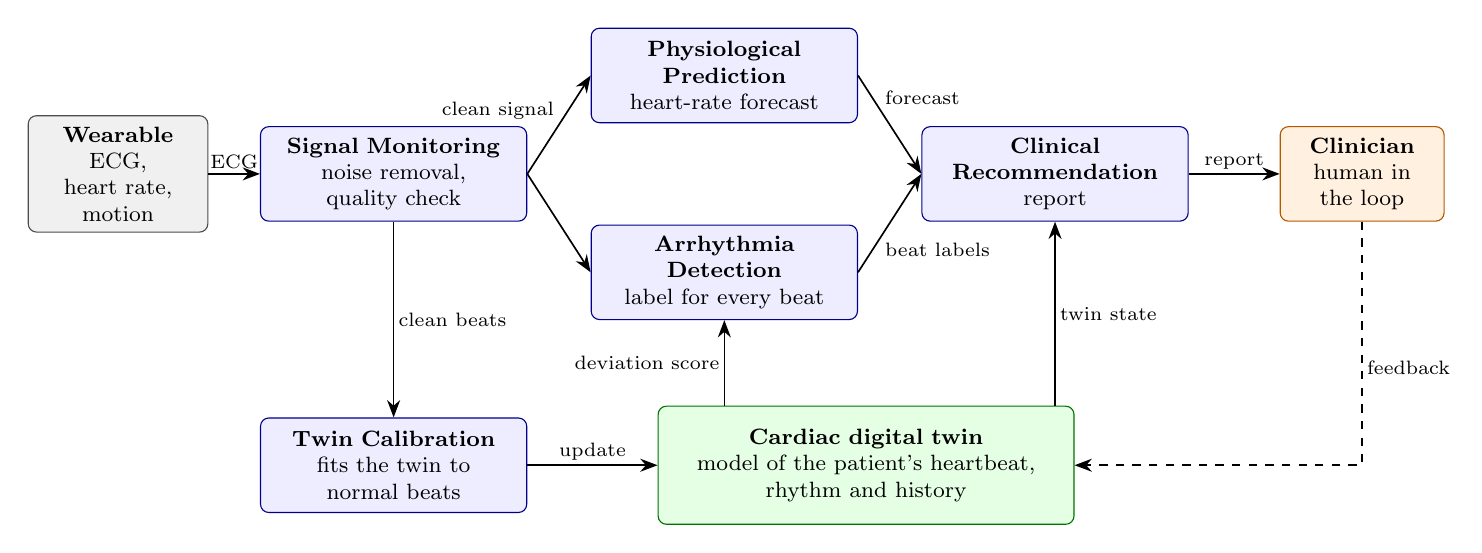
\begin{tikzpicture}[
  font=\footnotesize,
  box/.style={draw, rounded corners=3pt, align=center, inner sep=4pt, minimum height=12mm},
  io/.style={box, fill=gray!12, draw=gray!60!black, text width=20mm},
  agent/.style={box, fill=blue!7, draw=blue!55!black, text width=31mm},
  twinbox/.style={box, fill=green!10, draw=green!45!black, text width=50mm, minimum height=15mm},
  human/.style={box, fill=orange!12, draw=orange!70!black, text width=18mm},
  arr/.style={-{Stealth[length=2.2mm]}, semithick},
  lab/.style={font=\scriptsize, inner sep=1.5pt},
]
\node[io] (wear) at (0,0) {\textbf{Wearable}\\ECG, heart rate,\\motion};
\node[agent] (mon) at (3.5,0) {\textbf{Signal Monitoring}\\noise removal,\\quality check};
\node[agent] (pred) at (7.7,1.25) {\textbf{Physiological}\\\textbf{Prediction}\\heart-rate forecast};
\node[agent] (arr) at (7.7,-1.25) {\textbf{Arrhythmia}\\\textbf{Detection}\\label for every beat};
\node[agent] (rec) at (11.9,0) {\textbf{Clinical}\\\textbf{Recommendation}\\report};
\node[human] (clin) at (15.8,0) {\textbf{Clinician}\\human in\\the loop};
\node[agent] (cal) at (3.5,-3.7) {\textbf{Twin Calibration}\\fits the twin to\\normal beats};
\node[twinbox] (twin) at (9.5,-3.7) {\textbf{Cardiac digital twin}\\model of the patient's heartbeat,\\rhythm and history};

\draw[arr] (wear) -- node[lab, above]{ECG} (mon);
\draw[arr] (mon.east) -- node[lab, above left, pos=0.5]{clean signal} (pred.west);
\draw[arr] (mon.east) -- (arr.west);
\draw[arr] (mon.south) -- node[lab, right]{clean beats} (cal.north);
\draw[arr] (cal) -- node[lab, above]{update} (twin);
\draw[arr] (arr.south |- twin.north) -- node[lab, left]{deviation score} (arr.south);
\draw[arr] (pred.east) -- node[lab, above right, pos=0.35]{forecast} (rec.west);
\draw[arr] (arr.east) -- node[lab, below right, pos=0.35]{beat labels} (rec.west);
\draw[arr] (rec.south |- twin.north) -- node[lab, right]{twin state} (rec.south);
\draw[arr] (rec) -- node[lab, above]{report} (clin);
\draw[arr, dashed] (clin.south) |- node[lab, right, pos=0.3]{feedback} (twin.east);
\end{tikzpicture}}
\captionof{figure}{Graphical abstract: five agents share a model of the patient's heart (the twin); the clinician's feedback updates it.}
\label{fig:graphicalAbstract}
\end{center}


\chapter{State of the art/Related work}
\label{chapter:stateOfArt}

We searched Crossref, Semantic Scholar, OpenAlex, PubMed and the web for work in the five areas below, covering seminal papers and recent (2022--2026) ones.

\section{Cardiac digital twins}
\label{sec:rw-twins}

Corral-Acero et al.~\cite{corralacero2020digital} define the healthcare digital twin as a tool that integrates an individual's data over time using mechanistic and statistical models, and envision twins fed by wearable data. Niederer et al.~\cite{niederer2021scaling} note that current twins are bespoke and hard to scale. Coorey et al.~\cite{coorey2022health} require bidirectional data exchange with the patient; their review of 88 papers found that existing cardiovascular ``twins'' were simulation models, not real-time systems.

Most implemented twins are biophysical. Gillette et al.~\cite{gillette2021framework} fit a patient's anatomy to MR images and electrophysiology parameters to a 12-lead ECG; functional twinning was shown for a single subject. Simonian et al.~\cite{simonian2025development} build an image-based mitral-valve twin to predict the outcome of valve repair. Thangaraj et al.~\cite{thangaraj2024cardiovascular} describe hybrid twins that combine physiological parameters with lightweight deep learning, and point to smartwatches as a way to close the loop with the patient. Roop et al.~\cite{roop2025tuning} personalise a hybrid-automata model of the conduction system from wearable signals, and the ``Cardio Twin'' \cite{martinezvelazquez2019cardio} is an edge CNN that detects ischaemic heart disease from ECG (85.77\% accuracy).

\paragraph{Difference.} Our twin is a 15-parameter ECG model calibrated from one wearable lead, much cheaper than a biophysical twin. Unlike the Cardio Twin, it is a personalised model rather than a classifier, and clinician feedback flows back into it.

\section{Wearable ECG, signal quality and denoising}
\label{sec:rw-wearables}

Bayoumy et al.~\cite{bayoumy2021smart} find single-lead ECG useful for common arrhythmias such as AF but not for complex arrhythmias or infarction. In the Apple Heart Study \cite{perez2019large}, 0.52\% of 419,297 participants received an irregular-pulse notification; 34\% of those who returned an ECG patch had AF, and patches were applied on average 13 days after the notification. Bhavsar et al.~\cite{bhavsar2021digital} treat wearable measurements as digital biomarkers and add them to clinical reports. Del-Valle-Soto et al.~\cite{delvallesoto2024unveiling} survey biometric uses of wearables and stress privacy and data security.

Satija et al.~\cite{satija2018review} review ECG quality assessment and call for lightweight real-time methods for wearables. Smital et al.~\cite{smital2020realtime} grade quality continuously into three levels (full waveform, QRS only, unusable). Denoisers are usually tested on the MIT-BIH Noise Stress Test Database, where electrode-motion noise is hardest because it can mimic ectopic beats \cite{moody1984noise}. Sameni et al.~\cite{sameni2007nonlinear} use a dynamical ECG model inside Kalman filters, beating band-pass, adaptive and wavelet filtering. Learned alternatives include a convolutional denoising autoencoder \cite{chiang2019noise} and the diffusion model DeScoD-ECG \cite{li2024descod}.

\paragraph{Difference.} We combine a learned denoiser with graded quality levels \cite{smital2020realtime} and evaluate both by their effect on arrhythmia detection, not in isolation.

\section{Arrhythmia classification}
\label{sec:rw-classification}

The MIT-BIH Arrhythmia Database has 48 two-channel half-hour recordings from 47 subjects at 360~Hz \cite{moody2001impact}, and the AAMI EC57 standard defines how detectors are tested, with beat classes N, S, V, F and Q \cite{aami2013testing}. De Chazal et al.~\cite{dechazal2004automatic} introduced the inter-patient split; their feature-based classifier reached only 38.5\% positive predictivity on supraventricular beats. Kiranyaz et al.~\cite{kiranyaz2016realtime} train a small 1-D CNN per patient on common data plus the patient's own beats.

Hannun et al.~\cite{hannun2019cardiologist} classify 12 rhythm classes from single-lead ambulatory ECG with a mean ROC AUC of 0.97. Strodthoff et al.~\cite{strodthoff2021deep} benchmark models on PTB-XL, where ResNet- and Inception-style CNNs perform best. ECGFounder \cite{li2025electrocardiogram}, trained on about 10.8 million ECGs, has been adapted to single-lead recordings. Kapoor and Narayanan \cite{kapoor2023leakage} show that using the same patient in training and test data inflates results.

\paragraph{Difference.} We keep a population classifier with a strict inter-patient split. Instead of training a model per patient \cite{kiranyaz2016realtime}, we add the twin's deviation score $d_k$, which needs no labels from the new patient.

\section{Physiological ECG models and forecasting}
\label{sec:rw-models}

McSharry et al.~\cite{mcsharry2003dynamical} proposed the dynamical model behind our twin (Eq.~\eqref{eq:ecgsyn}). Clifford et al.~\cite{clifford2005model} fit it to each beat for patient-specific filtering and beat clustering, treating beats the model cannot fit as artefacts. Sayadi et al.~\cite{sayadi2010robust} track ECG waves with a model-based Kalman filter and detect premature ventricular contractions from the filter's output (99.10\% accuracy).

For forecasting, the Temporal Fusion Transformer \cite{lim2021temporal} gives interpretable multi-horizon forecasts and PatchTST \cite{nie2023time} uses patches of the series as tokens. A one-layer linear model nevertheless beat Transformer forecasters on nine datasets \cite{zeng2023transformers}, and for wearable heart rate a linear autoregressive model beat LSTMs \cite{staffini2021heart}.

\paragraph{Difference.} We keep the fitted parameters as a persistent twin state that other agents query, and treat beats the model cannot fit as candidate abnormal beats rather than artefacts. Forecasters must beat persistence and autoregressive baselines.

\section{LLM agents for health monitoring}
\label{sec:rw-agents}

ReAct \cite{yao2023react} interleaves reasoning with tool calls. MDAgents \cite{kim2024mdagents} assigns one model or a group of models to a medical task depending on its complexity and was best on 7 of 10 medical benchmarks. PHIA \cite{merrill2026transforming} analyses wearable data through code generation and retrieval, with 84\% accuracy on numerical questions. Hager et al.~\cite{hager2024evaluation} found that LLMs diagnosed 2,400 real cases significantly worse than physicians and are not ready for autonomous decisions.

\paragraph{Difference.} Our agents orchestrate validated signal models and write reports; they do not diagnose, and a clinician reviews every report.

\section{Positioning}
\label{sec:rw-positioning}

Table~\ref{tab:positioning} compares representative works. We found no work that combines single-lead wearable input, a calibrated patient-specific ECG model, learned detection and an agent layer.

\begin{table}[htbp]
\caption{Comparison with related work ($\checkmark$: stated in the cited work).}
\label{tab:positioning}
\centering
\footnotesize
\setstretch{1.1}
\newcommand{\y}{$\checkmark$}
\setlength{\tabcolsep}{4pt}
\begin{tabular}{@{}lcccccc@{}}
\toprule
\textbf{Work} & \textbf{\shortstack{Single-lead /\\wearable}} & \textbf{\shortstack{Patient-\\specific}} & \textbf{\shortstack{Physiological\\model}} & \textbf{\shortstack{Deep\\learning}} & \textbf{\shortstack{Arrhythmia\\detection}} & \textbf{\shortstack{LLM\\agents}} \\
\midrule
Gillette et al.~\cite{gillette2021framework} & & \y & \y & & & \\
Roop et al.~\cite{roop2025tuning} & \y & \y & \y & & & \\
Martinez-Velazquez et al.~\cite{martinezvelazquez2019cardio} & & & & \y & & \\
Clifford et al.~\cite{clifford2005model} & \y & \y & \y & & \y & \\
Sayadi et al.~\cite{sayadi2010robust} & \y & & \y & & \y & \\
Kiranyaz et al.~\cite{kiranyaz2016realtime} & \y & \y & & \y & \y & \\
Hannun et al.~\cite{hannun2019cardiologist} & \y & & & \y & \y & \\
Merrill et al.~\cite{merrill2026transforming} & \y & & & & & \y \\
\midrule
\textbf{This project} & \y & \y & \y & \y & \y & \y \\
\bottomrule
\end{tabular}
\end{table}

\chapter{Conclusion and future work}
\label{chapter:concl}

Next steps:
\begin{itemize}
	\item \textbf{Seminar 4:} exploratory analysis of the MIT-BIH Arrhythmia and Noise Stress Test databases; first denoiser, inter-patient classifier and forecasting baselines; twin calibration on real beats.
	\item \textbf{Seminar 6:} agent orchestration and clinical reports; classifier with vs.\ without the deviation score $d_k$.
	\item \textbf{Seminar 7:} deployed application, SWOT analysis and presentation.
\end{itemize}


\bibliographystyle{plainurl}
{\small\setstretch{1.0}\bibliography{references}}

\end{document}
